\documentclass[aspectratio=169,11pt]{beamer}
\usetheme{metropolis}

\usepackage{fontspec}
\defaultfontfeatures{Ligatures=TeX}
\setmainfont{Latin Modern Roman}
\setsansfont{Latin Modern Sans}
\setmonofont{Latin Modern Mono}
\usepackage{amsmath, amssymb}
\usepackage{booktabs}
\usepackage{tikz}
\usetikzlibrary{arrows.meta, positioning, shapes.geometric}
\usepackage{xcolor}

\definecolor{mDarkTeal}{HTML}{23373B}
\definecolor{mLightBlue}{HTML}{4F9DA6}
\definecolor{mLightGreen}{HTML}{7EC8A9}
\definecolor{mLightBrown}{HTML}{D7B49E}

\setbeamertemplate{caption}[numbered]
\setbeamerfont{footnote}{size=\tiny}
\setbeamertemplate{itemize items}[circle]
\setbeamertemplate{enumerate items}[default]

\title{Conditional Entropy Defenses with Attention}
\subtitle{Slot + Gated Cross Attention vs. Gated Attention Pooling}
\author{Project Update}
\date{Group Meeting Preparation}
\institute{Attention Privacy Project}

\newcommand{\highlight}[1]{\textcolor{mDarkTeal}{\textbf{#1}}}

\begin{document}

\begin{frame}[plain]
  \titlepage
\end{frame}

\begin{frame}{Roadmap}
  \begin{itemize}
    \item Recap: collaborative inference threat model and CEM requirements
    \item Slot + Gated Cross Attention surrogate
    \item Gated Attention Pooling surrogate
    \item Comparison, monitoring guidance, next steps
  \end{itemize}
\end{frame}

\section{Background}

\begin{frame}{Collaborative Inference \& CEM Goal}
  \begin{columns}[T]
    \begin{column}{0.55\textwidth}
      \begin{itemize}
        \item Local encoder $F_e$ uploads feature vectors $z$ to the cloud decoder $F_d$; attacker can attempt input reconstruction.
        \item Conditional entropy maximization (CEM) seeks to keep $H(x \mid z)$ high so reconstructions remain uncertain.
        \item Legacy implementation used KMeans/GMM to approximate per-class variance and penalize sharp feature clusters.
        \item New attention surrogates replace GMM for richer class structure modeling while remaining differentiable.
      \end{itemize}
    \end{column}
    \begin{column}{0.4\textwidth}
      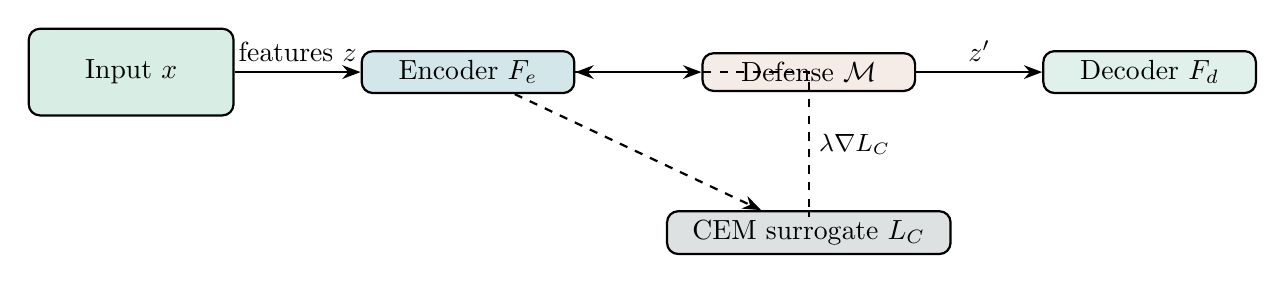
\begin{tikzpicture}[>=Stealth, thick, node distance=1.6cm]
        \node[draw, rounded corners, minimum width=2.6cm, minimum height=1.1cm, fill=mLightGreen!30] (input) {Input $x$};
        \node[draw, rounded corners, right=of input, minimum width=2.7cm, fill=mLightBlue!25] (encoder) {Encoder $F_e$};
        \node[draw, rounded corners, right=of encoder, minimum width=2.7cm, fill=mLightBrown!25] (defense) {Defense $\mathcal{M}$};
        \node[draw, rounded corners, right=of defense, minimum width=2.7cm, fill=mLightGreen!25] (decoder) {Decoder $F_d$};
        \node[draw, rounded corners, below=1.5cm of defense, minimum width=3.6cm, fill=mDarkTeal!15] (cem) {CEM surrogate $L_C$};
        \draw[->] (input) -- (encoder) node[midway, above]{features $z$};
        \draw[->] (encoder) -- (defense);
        \draw[->] (defense) -- node[midway, above]{$z'$} (decoder);
        \draw[->, dashed] (encoder) -- (cem);
        \draw[->, dashed] (cem) -- ++(0,0.2) |- (encoder) node[pos=0.25, right]{\small $\lambda \nabla L_C$};
      \end{tikzpicture}
    \end{column}
  \end{columns}
\end{frame}

\begin{frame}{Design Criteria for Attention CEM}
  \begin{itemize}
    \item \highlight{Fine-grained}: capture multi-modal subclasses within each label instead of assuming a single Gaussian.
    \item \highlight{Stable}: avoid exploding gradients and NaNs; guard against small batches or class imbalance.
    \item \highlight{Optimizer-friendly}: expose gradients that can be merged with encoder updates via $\lambda$.
    \item \highlight{Diagnostics}: surface interpretable statistics (slot gates, SNR signals, variance margins) to guide tuning.
  \end{itemize}
\end{frame}

\section{Slot + Gated Cross Attention}

\begin{frame}{Pipeline Overview}
  \begin{center}
    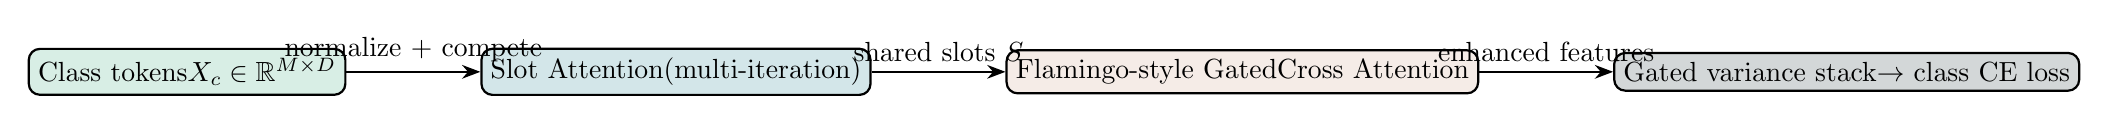
\begin{tikzpicture}[>=Stealth, thick, node distance=1.7cm]
      \node[draw, rounded corners, minimum width=3.3cm, fill=mLightGreen!30] (tokens) {Class tokens\\$X_c \in \mathbb{R}^{M \times D}$};
      \node[draw, rounded corners, right=of tokens, minimum width=3.4cm, fill=mLightBlue!25] (slot) {Slot Attention\\(multi-iteration)};
      \node[draw, rounded corners, right=of slot, minimum width=3.7cm, fill=mLightBrown!25] (cross) {Flamingo-style Gated\\Cross Attention};
      \node[draw, rounded corners, right=of cross, minimum width=4.2cm, fill=mDarkTeal!20] (gates) {Gated variance stack\\$\rightarrow$ class CE loss};
      \draw[->] (tokens) -- node[above]{normalize + compete} (slot);
      \draw[->] (slot) -- node[above]{shared slots $S$} (cross);
      \draw[->] (cross) -- node[above]{enhanced features} (gates);
    \end{tikzpicture}
  \end{center}
  \begin{itemize}
    \item Processes one class at a time; reuses slots to encode latent sub-modes.
    \item Cross attention re-injects slot context into every sample before measuring dispersion.
  \end{itemize}
\end{frame}

\begin{frame}{Slot Attention Core (Locatello et al.)}
  \begin{itemize}
    \item Inputs are LayerNormed and projected to keys/values once per class.
    \item Slots are initialized from a learned Gaussian $(\mu, \sigma)$ and iteratively refined ($T{=}3$).
    \item Competitive soft assignments $r_{ms} = \text{softmax}(\beta \, \text{sim}(x_m,s_s))$ ensure each slot explains part of the class.
    \item GRU + MLP residual updates preserve temporal dynamics and stabilize slot representations.
    \item Learnable temperature $\beta$ and slot sharpening power adjust how concentrated each slot becomes.
  \end{itemize}
\end{frame}

\begin{frame}{Flamingo-Style Gated Cross Attention}
  \begin{itemize}
    \item Pre-LN multi-head cross attention (4 heads) with learnable $\alpha_{\text{attn}}$ gate:
      \[
        y = q + \tanh(\alpha_{\text{attn}}) \cdot \mathrm{CrossAttn}(q, s).
      \]
    \item Feed-forward block mirrors Flamingo dense layer with a second gate $\alpha_{\text{ffn}}$ for gradual activation.
    \item Slots act as shared KV memory; query tokens are the LayerNormed class samples.
    \item Dropout-free path keeps gradients deterministic, easing debugging.
  \end{itemize}
\end{frame}

\begin{frame}{Conditional Entropy Surrogate}
  \small
  \begin{enumerate}
    \item \highlight{Mixture-of-slots variance}: compute per-slot mean $\mu_s$ and variance $\sigma_s^2$ under sharpened responsibilities.
    \item \highlight{Per-dimension gate}: $\text{sigmoid}(\mathrm{MLP}(\mathrm{LN}(\log \sigma_s^2)))$ suppresses low-signal dimensions.
    \item \highlight{SNR gate}: $\sigma(\kappa(\sigma_s^2 / (\mu_s^2 + \epsilon) - \tau))$ dampens high-SNR activations that leak semantics.
    \item \highlight{Softplus margin}: $L_{\text{base}} = \frac{1}{\beta'} \log\!\big(1 + e^{\beta'(\log \sigma_s^2 - \log \tau - m)}\big)$ smooths the hinge at the variance threshold.
    \item \highlight{Slot mass weighting}: responsibilities are sharpened by $w_s \propto (\text{mass}_s/M)^{\rho}$ to focus on dominant slots.
    \item \highlight{Class gate}: $g_c = \sigma(a(M/B - b))$ scales classes with scant samples to avoid noisy penalties.
  \end{enumerate}
\end{frame}

\begin{frame}{Training Integration \& Safety Nets}
  \begin{itemize}
    \item Activation: only after warmup ($>3$ epochs), non-random centers, and $\lambda>0$.
    \item Gradients: backprop through $L_C$, stash encoder gradients, zero optimizers, then blend with classification gradients using $\lambda$ and LR-aware rescaling.
    \item Scaling: final $L_C$ contribution multiplied by $\texttt{attention\_loss\_scale}=0.25$ before gradient capture.
    \item Early shutoff: for first 100 calls or when gate statistics exceed thresholds, $L_C$ returns a graph-connected zero to avoid destabilizing the encoder.
    \item Robustness: skip computation if NaN/Inf features, and lazily register module parameters into the optimizer only once.
    \item Logging: prints mean gate activations and slot statistics every 200 calls to guide hyper-parameter tuning.
  \end{itemize}
\end{frame}

\section{Gated Attention Pooling}

\begin{frame}{Why a Second Surrogate?}
  \begin{itemize}
    \item Slot pipeline is expressive but heavy: GRUs, multi-head attention, and numerous gates increase flops and tuning cost.
    \item Need a lightweight alternative for large batches, high-resolution encoders, or quick ablations.
    \item Gated Attention Pooling borrows from deep MIL: a single attention distribution summarizes class features.
  \end{itemize}
\end{frame}

\begin{frame}{Pooling Architecture}
  \begin{center}
    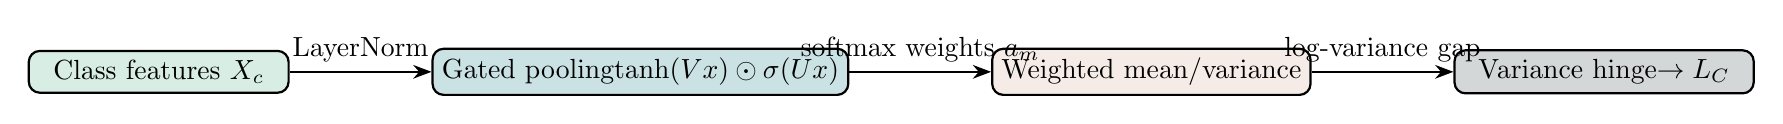
\begin{tikzpicture}[>=Stealth, thick, node distance=1.8cm]
      \node[draw, rounded corners, minimum width=3.3cm, fill=mLightGreen!30] (tokens) {Class features $X_c$};
      \node[draw, rounded corners, right=of tokens, minimum width=3.5cm, fill=mLightBlue!30] (gate) {Gated pooling\\$\tanh(Vx)\odot\sigma(Ux)$};
      \node[draw, rounded corners, right=of gate, minimum width=3.6cm, fill=mLightBrown!25] (stats) {Weighted mean/variance};
      \node[draw, rounded corners, right=of stats, minimum width=3.8cm, fill=mDarkTeal!20] (loss) {Variance hinge\\$\rightarrow L_C$};
      \draw[->] (tokens) -- node[above]{LayerNorm} (gate);
      \draw[->] (gate) -- node[above]{softmax weights $a_m$} (stats);
      \draw[->] (stats) -- node[above]{log-variance gap} (loss);
    \end{tikzpicture}
  \end{center}
\end{frame}

\begin{frame}{Mathematics}
  \small
  \begin{align*}
    a_m &= \frac{\exp\big(w^\top[\tanh(Vx_m)\odot\sigma(Ux_m)]\big)}{\sum_j \exp(\cdot)}, \\
    \mu_c &= \sum_m a_m x_m, \qquad
    \sigma_c^2 = \sum_m a_m (x_m - \mu_c)^2, \\
    \tau &= \texttt{var\_threshold} \cdot \texttt{reg\_strength}^2 + \gamma, \\
    L_C &= \max\!\left\{0,\, \log(\sigma_c^2 + \gamma) - \log(\tau)\right\}.
  \end{align*}
  \vspace{-0.8em}
  \begin{itemize}
    \item LayerNorm of inputs curbs variance collapse under sharp attention distributions.
    \item Hidden size defaults to $\min(512, \max(64, D/4))$ per class at instantiation.
    \item ReLU-style hinge keeps gradients sparse when class variance already exceeds the target threshold.
  \end{itemize}
\end{frame}

\begin{frame}{Training Notes}
  \begin{itemize}
    \item Warmup extends to 5 epochs to let softmax weights stabilize.
    \item Module lazily constructed on first use and registered with the optimizer; gradients combined with encoder updates just like the slot version.
    \item Uses a smaller scaling factor: $\texttt{attention\_loss\_scale}=0.1$ before gradient capture.
    \item Skips classes with $\leq 1$ samples to avoid ill-defined variance; safe defaults return zero loss.
    \item Same guardrails for NaN/Inf detection and optimizer resets after the auxiliary backward pass.
  \end{itemize}
\end{frame}

\begin{frame}{When to Prefer Each}
  \begin{itemize}
    \item \highlight{Use Slot + Gated Cross Attention} when class heterogeneity is high (complex datasets, multi-modal privacy leakage) and logging bandwidth is available.
    \item \highlight{Use Gated Attention Pooling} for rapid experimentation, limited compute, or when you mainly need coarse variance inflation.
    \item Both surrogates can be toggled via the training script; only one runs per experiment.
  \end{itemize}
\end{frame}

\section{Comparison \& Next Steps}

\begin{frame}{Side-by-Side Summary}
  \begin{table}
    \centering
    \begin{tabular}{p{3.2cm}p{4.8cm}p{4.8cm}}
      \toprule
      & \textbf{Slot + Gated Cross Attn} & \textbf{Gated Attention Pooling} \\
      \midrule
      Representation & Multi-slot latent mixture with cross-attention refinement & Single attention distribution over class tokens \\
      Gates & Per-dim MLP, SNR gate, slot mass, class gate, softplus margin & Single gated attention + variance hinge \\
      Compute & GRU iterations + multi-head attention (heavier) & Two linear layers + softmax (light) \\
      Tuning knobs & $\beta$, slot power, SNR threshold, class gate bias, margin & Threshold $\tau$, loss scale, hidden width \\
      Safety & Early shutoff, extensive logging, NaN guards & Skip small classes, automatic hidden size \\
      \bottomrule
    \end{tabular}
  \end{table}
\end{frame}

\begin{frame}{Operational Guidance}
  \begin{itemize}
    \item Monitor: slot gate means, hard gate averages, and class-level activations printed by the module; large values signal over-sharpening.
    \item For Gated Pooling, track variance histograms versus $\tau$ to ensure the hinge is active for risky classes.
    \item Adjust $\lambda$ schedule alongside $\texttt{attention\_loss\_scale}$ to balance accuracy and privacy cost.
    \item Remember to rerun validation with reconstruction attacks after enabling either surrogate to quantify impact.
  \end{itemize}
\end{frame}

\begin{frame}[plain]
  \centering\Huge Thank you!
\end{frame}

\end{document}
